%% Based on a TeXnicCenter-Template by Gyorgy SZEIDL.
%%%%%%%%%%%%%%%%%%%%%%%%%%%%%%%%%%%%%%%%%%%%%%%%%%%%%%%%%%%%%

%------------------------------------------------------------
%
\documentclass[letterpaper,10pt]{article}
%
\usepackage{amsmath}%
\usepackage{amsfonts}%
\usepackage{amssymb}%
\usepackage{graphicx}
%-------------------------------------------
\newtheorem{theorem}{Theorem}
\newtheorem{acknowledgement}[theorem]{Acknowledgement}
\newtheorem{algorithm}[theorem]{Algorithm}
\newtheorem{axiom}[theorem]{Axiom}
\newtheorem{case}[theorem]{Case}
\newtheorem{claim}[theorem]{Claim}
\newtheorem{conclusion}[theorem]{Conclusion}
\newtheorem{condition}[theorem]{Condition}
\newtheorem{conjecture}[theorem]{Conjecture}
\newtheorem{corollary}[theorem]{Corollary}
\newtheorem{criterion}[theorem]{Criterion}
\newtheorem{definition}[theorem]{Definition}
\newtheorem{example}[theorem]{Example}
\newtheorem{exercise}[theorem]{Exercise}
\newtheorem{lemma}[theorem]{Lemma}
\newtheorem{notation}[theorem]{Notation}
\newtheorem{problem}[theorem]{Problem}
\newtheorem{proposition}[theorem]{Proposition}
\newtheorem{remark}[theorem]{Remark}
\newtheorem{solution}[theorem]{Solution}
\newtheorem{summary}[theorem]{Summary}
\newenvironment{proof}[1][Proof]{\textbf{#1.} }{\ \rule{0.5em}{0.5em}}

% Construct the basic page sizes
\oddsidemargin  0.0in
\evensidemargin 0.0in
\textwidth      6.5in
\headheight     0.25in
\topmargin      0.0in
\textheight=8.5in

\begin{document}

\title{Using GMAT's C Interface Library\\\large{Revision 0.01, ODTBX Instructions}}
\author{Darrel J. Conway\thanks{Developed under Prime Contract NNG10CP02C, Task Order 28.}
\\Thinking Systems, Inc.}
\date{\today}
\maketitle

\begin{abstract}
This document describes how to use GMAT's C-interface.  It includes descriptions of the methods currently implemented and examples of the calls into the interface made from MATLAB.  It also includes a section showing how to use the interface from ODTBX. 
\end{abstract}

\section{Introduction}

The General Mission Analysis Tool, GMAT, is a space trajectory optimization and mission analysis system developed by NASA and private industry in the spirit of the NASA Vision. GMAT contains new technology and is a testbed for future technology development. One way GMAT provides testbed capabilities is through a library designed to access part of the system's features using calls to C functions.  This document describes that interface.

GMAT is coded in C++ using modern, object oriented design principles.  The implementation of the system in C++ provides challenges for systems written in other languages that want to access GMAT components.  The C interface described here overcomes some of these difficulties by providing simpler calls into GMAT than would be possible if the class structures were accessed directly.  This functionality is limited to the components that have been exposed through the interface.  GMAT's C interface currently provides access to a small subset of the total system, but has been designed to be extended to other components as needed.  The full set of currently implemented elements is provided in Appendix~\ref{sec:FunctionList}.

The following sections describe how to configure a computer to use the C interface, how to make calls into GMAT from MATLAB, and provide an example of the call into GMAT's ODE model for use in an ODTBX integrator.

\section{Setting up the Environment}

GMAT's C interface is implemented as a plugin library that provides access to GMAT objects through C functions.  The library starts a copy of GMAT's engine, loads a configuration by means of a GMAT script, populates a GMAT Sandbox with the configuration, and then provides access to the objects in the Sandbox.

\section{Accessing GMAT Objects from MATLAB}

\section{An ODTBX Example: Integrating an Orbit}

\appendix

\section{Data File Organization}

GMAT requires access to data files organized in a file structure described in the GMAT startup file, gmat\_startup\_file.txt.  That file should be in the working folder from which the interface is accessed.  In a typical setup, the GMAT startup file identifies a root folder, a data file folder, and then uses these tow locations to identify the locations of additional data files needed by GMAT.  A typical startup file contains these lines for the top level folders:

\begin{quote}
\begin{verbatim}
ROOT_PATH              = ../
DATA_PATH              = ROOT_PATH/data/
\end{verbatim}
\end{quote}

\noindent The remaining lines in the file describe the locations of planetary ephemerides, coefficient files for planetary gravity fields, time system data, and other data elements needed when GMAT runs.  A typical file structure for the data files is shown in Figure~\ref{fig:DataFileStrucure}.

\begin{figure}[htb]
  \begin{center}
	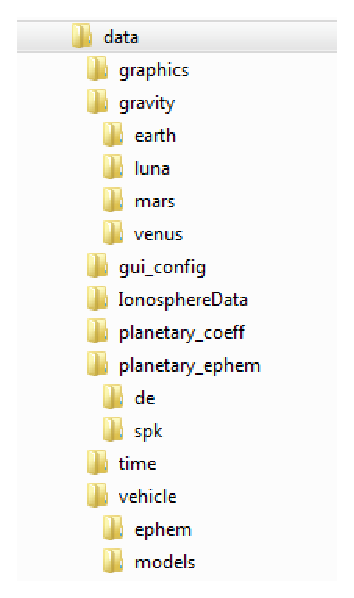
\includegraphics{Images/DataFileLayout.eps}
	\caption{The Default Data File Strucure for GMAT}
	\label{fig:DataFileStrucure}
  \end{center}
\end{figure}

\noindent This file structure matches the structure delivered with GMAT R2011a.  It also matches the data file structure found in the source code repository for GMAT at SourceForge at the time of this writing.  The entries in the GMAT startup file point to specific files in this structure.  For example, the lines

\begin{quote}
\begin{verbatim}
SPK_PATH               = DATA_PATH/planetary_ephem/spk/
PLANETARY_SPK_FILE     = SPK_PATH/de421.bsp
\end{verbatim}
\end{quote}

\noindent identify the location of the SPICE planetary ephemeris file, de421.bsp, in the file system.  Using the entries provided thus far, GMAT looks for the file

\begin{quote}
\begin{verbatim}
../data/planetary_ephem/spk/de421.bsp
\end{verbatim}
\end{quote}

\noindent relative to the starting folder for the system.  The startup file provides similar path data for all of GMAT's data files; interested users should look in this file when trying to understand the data used when running a mission.

\section{\label{sec:FunctionList}Supported Functions}

\end{document}
